\section{Wybrane aspekty realizacji}
\label{sec:wybrane-aspekty-realizacji}
Najmniejsza możliwa konfiguracja systemu to pojedynczy, samodzielnie działający
węzeł (magazyn danych). Węzeł jest aplikacją Erlang/OTP \cite{otp-www, otp-lyse} (spakowaną razem ze środowiskiem uruchomieniowym).

\subsection{Architektura systemu}
Węzły systemu są połączone między sobą (znają swoje adresy) w sieć tworzącą graf pełny. Finalna wersja architektury jest identyczna z tą przedstawioną na \autoref{fig:arch-overview}. Cała komunikacja między nimi oparta jest wyłącznie na komunikatach języka Erlang. Komunikaty, w zależności od typu, są rozgłaszane po całym systemie lub kierowane bezpośrednio do odpowiedniego węzła.

Każdy węzeł systemu zarządza pewnym podzbiorem wszystkich plików. Jeżeli do węzła trafia zapytanie dotyczące odczytu, usunięcia czy wyszukania pliku, zostanie rozesłane do wszystkich węzłów w systemie. Zapytania tworzące wymagają znalezienia optymalnej lokalizacji do przechowywania nowego pliku. Zapytanie takie nie jest rozgłaszane, lecz przekazywane bezpośrednio do docelowego węzła.

Za przesłanie odpowiedzi do użytkownikowa odpowiada zawsze tylko jeden węzeł - ten, który obsłużył zapytanie (przechowywał poszukiwany plik). Pozostałe węzły ignorują zapytania dotyczące plików, których nie posiadają. W przypadku nieotrzymania odpowiedzi po określonym czasie, przyjmuje się, że zapytanie zakończyło się niepowodzeniem (\textit{timeout}).

Użytkownik może wykonywać swoje zapytania na dowolnym z węzłów. Potrzebuje jedynie znać jego adres sieciowy (wraz z portem na jakim działa usługa HTTP). Niezależnie do którego węzła użytkownik skieruje zapytanie, zawsze otrzyma dostęp do wszystkich swoich plików. Informacja o fizycznej lokalizacji pliku jest widoczna w aplikacji webowej oraz obecna w odpowiedziach systemu na zapytania \textit{list} (lista plików) czy \textit{find} (wyszukanie pliku). Wybór węzła dostępowego (ang. \textit{gateway node}) nie powinien mieć wpływu na wydajność.

Kiedy nowy węzeł dołączany jest do systemu, pobiera informacje o pozostałych węzłach od jednego z nich (dowolnego, nazywanego \textit{initial node}), a następnie rozgłasza do wszystkich pozostałych węzłów komunikat o swoim dołączeniu.

\subsection{Struktura magazynu danych (węzła)}
Pojedynczy węzeł składa się gółwnego \textit{supervisora}, zarządzającego pracą pięciu komunikujących się \textit{gen\_serverów}: \textit{http\_srv}, \textit{auth\_srv}, \textit{dist\_srv}, \textit{core\_srv}, \textit{uuid\_srv}. Supervisor pracuje w polityce \textit{one-for-one}, co znaczy że w razie awarii każdy komponent będzie restartowany niezależnie od pozostałych.

Każdy z gen\_serverów ma jasno określone zadania. Poszczególne serwery (moduły) ściśle współpracują między sobą i wymieniają wiadomości w celu obsługi zapytania. Na podstawie przepływu informacji między nimi można wyróżnić warstwową hierarchię przedstawioną na \autoref{fig:node-structure}.

\begin{figure}[!htbp]
	\centering
	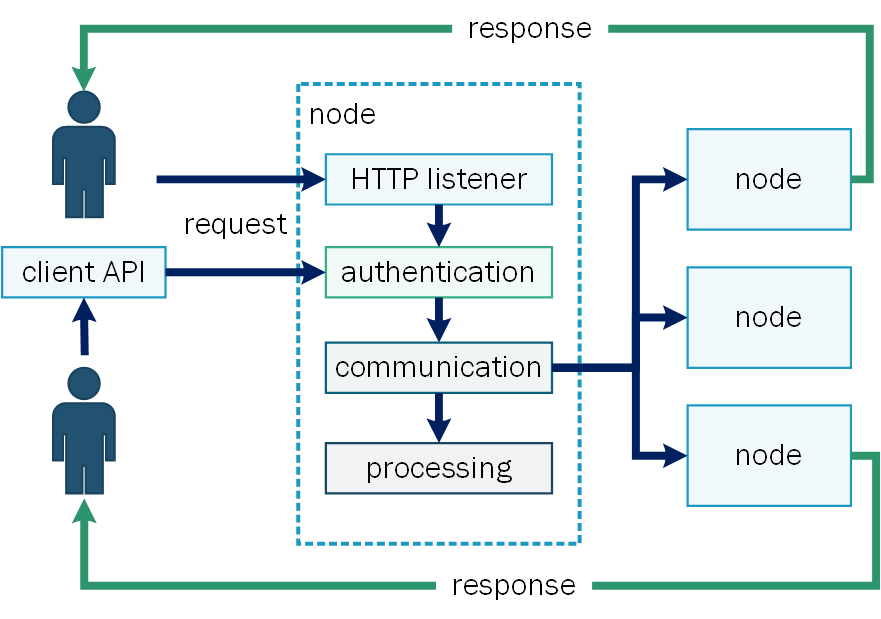
\includegraphics[width=0.6\textwidth]{images/fig02-node-structure.png}
	\caption{Przepływ zapytań w węźle systemu.}
	\label{fig:node-structure}
\end{figure}

\paragraph{http\_srv:} Moduł opcjonalny, jego obecność nie jest wymagana do poprawnej pracy całego systemu. Moduł służy do przetwarzania zapytań HTTP i generowania odpowiedzi. Potrafi również serwować statyczne pliki HTML – przykładowo graficzny menedżer plików. Standardowo, dostęp do systemu odbywa się poprzez ten właśnie moduł, przy użyciu oferowanego REST API.

\paragraph{auth\_srv:} Moduł autentykacji odpowiada za obliczanie i weryfikację sumy kontrolnej HMAC przekazywanych zapytań. Zarządza również lokalną dla danego węzła pamięcią podręczną użytkowników (ang. \textit{cache}).

\paragraph{dist\_srv:} Jest to moduł odpowiedzialny za komunikację między węzłami systemu. Zapytania są autentykowane (z użyciem \textit{auth\_srv}) a następnie przesyłane dalej zgodnie z polityką obsługi danego typu zapytania. Moduł ten odpowiada również obsługę dołączania do systemu nowych węzłów.

\paragraph{core\_srv:} Moduł \textit{core} to główny moduł logiki systemu, odpowiedzialny za realizację wszystkich zleconych operacji. Komunikuje się bezpośrednio z bazą danych i systemem plików. Tutaj trafiają wszystkie zapytania w finalnej fazie obsługi. Odpowiedzi kierowane są zwykle wprost do użytkownika. Wewnątrz można wyróżnić dwa elementy: pulę wątków wykonawczych, przetwarzających zapytania i realizujących operacje I/O oraz wątek schedulera, zarządzający kolejnością uruchamiania wątków wykonawczych.

\paragraph{uuid\_srv:} Jest to wielowątkowy moduł służący do generowania unikalnych, 128-bitowych identyfikatorów \cite{snowflake}. Identyfikatory te są wykorzystywane jako nazwy fizycznych plików przechowywanych w systemie dyskowym. Właściwymi identyfikatorami plików i użytkowników w systemie pozostają jednak zwykłe napisy, w postaci czytelnej dla człowieka. Identyfikator składa się z trzech części – grup bitów, z których każda ma odpowiednią interpretację:
\centerline{\texttt{<< 48bit timestamp, 48bit adres MAC, 32bit losowa wartość >>}}

\subsection{Baza danych}
System korzysta z bazy danych SQLite3 \cite{sqlite-www}. Dla naszych zastosowań okazała się najwydajniejsza spośród dostępnych baz danych \cite{sqlite-perf}. Z powodzeniem uruchomiliśmy również konfigurację z bazą MySQL, jednak wymagała więcej konfiguracji i oferowała niższą wydajność.

W bazie danych persystowane są trzy rodzaje struktur: \textit{User}, \textit{File} oraz \textit{Action}.

\paragraph{User:} Struktura opisująca użytkownika systemu. Podstawowe pola to login, skrót hasła - klucza (\textit{secret}) oraz data utworzenia konta.

\paragraph{File:} Metadane dotyczące pliku:
\begin{itemize}
	\item nazwa - tekstowy identyfikator pliku. Nazwy plików jednego właściciela muszą być unikatowe. Interpretując system jako bazę klucz-wartość, nazwa pliku jest kluczem (a zawartość obiektem)
	\item właściciel - identyfikator osoby, która utworzyła plik. Właściciel ma pełne prawa dostępu do pliku
	\item rozmiar - rozmiar pliku w bajtach. Pliki o większym rozmiarze mają większy koszt przetwarzania
	\item data utworzenia
	\item data ostatniego dostępu
\end{itemize}

\paragraph{Action:} Informacja o przetworzeniu zapytania użytkownika. Gromadzone do celów statystycznych, zawierają takie dane jak typ operacji czy wagę żądanego pliku.

\subsection{Autentykacja}
Autentykacja bazuje na sumie kontrolnej HMAC \cite{hmac-art}. keyed-Hash Message Authentication Code to funkcja skrótu z dodatkowo wmieszanym kluczem prywatnym. Wynikowy kod zależy nie tylko od danych z których jest obliczany, ale również od wykorzystanego hasła. Hasło (klucz prywatny) znane jest tylko użytkownikowi oraz systemowi. Nie jest przesyłane między nimi, co zmniejsza szanse na ujawnienie klucza.

Wykorzystanie HMAC zapewnia ochronę integralności przesyłanych zapytań (modyfikacja parametrów zapytania wymaga przeliczenia sumy HMAC) oraz autentyczności danych (wyliczenie sumy wymaga znajomości klucza prywatnego).

Każdy użytkownik posiada "hasło" (ang. \textit{secret}). Może on je ustalić dowolnie ze swoimi preferencjami. Kluczem prywatnym staje się suma SHA1 obliczona z tego hasła, i tylko ta wartość przechowywana jest w bazie danych.

\subsection{Scheduling}
Scheduler jest modułem szeregującym zapytania trafiające do danego węzła. Zarządza on pulą wątków wykonawczych (ang. \textit{executor}), odpowiedzialnych za bezpośrednią obsługę zadań. Każdy plik (każda ścieżka) ma przydzielony jeden wątek wykonawczy. Zapytania dotyczące konkretnego pliku zawsze więc są obsługiwane przez jeden wątek.
Scheduler umieszcza wszystkie przychodzące akcje w kolejce priorytetowej. Przed rozpoczęciem przetwarzania kolejnego zadania, wątek wykonawczy czeka na pozwolenie od schedulera. Po każdym zakończonym zadaniu informuje scheduler o zakończeniu jego obsługi.

\begin{figure}[!htbp]
	\centering
	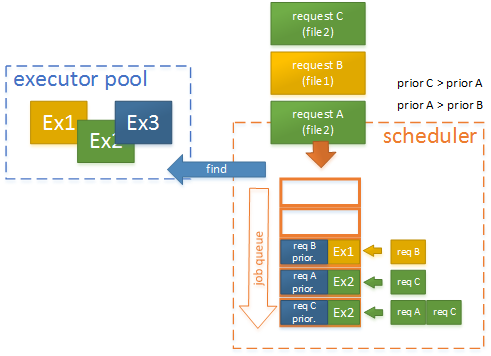
\includegraphics[width=0.8\textwidth]{images/fig03-scheduler.png}
	\caption[Schemat działania schedulera.]{Schemat działania schedulera. Zapytania są parowane z priorytetami, tworząc \textit{akcje}. Takie akcje trafiają do kolejki, gdzie czekają na uruchomienie.}
	\label{fig:scheduler}
\end{figure}

Scheduler uruchamia N (domyślnie 4) pierwszych wątków wykonawczych z kolejki priorytetowej. Jeżeli jakiś wątek skończy przetwarzać jakieś zapytanie, scheduler wybiera z kolejki w jego miejsce wątek o najwyższym priorytecie.
